% Options for packages loaded elsewhere
% Options for packages loaded elsewhere
\PassOptionsToPackage{unicode}{hyperref}
\PassOptionsToPackage{hyphens}{url}
%
\documentclass[
  ignorenonframetext,
  aspectratio=169,
]{beamer}
\newif\ifbibliography
\usepackage{pgfpages}
\setbeamertemplate{caption}[numbered]
\setbeamertemplate{caption label separator}{: }
\setbeamercolor{caption name}{fg=normal text.fg}
\beamertemplatenavigationsymbolsempty
% remove section numbering
\setbeamertemplate{part page}{
  \centering
  \begin{beamercolorbox}[sep=16pt,center]{part title}
    \usebeamerfont{part title}\insertpart\par
  \end{beamercolorbox}
}
\setbeamertemplate{section page}{
  \centering
  \begin{beamercolorbox}[sep=12pt,center]{section title}
    \usebeamerfont{section title}\insertsection\par
  \end{beamercolorbox}
}
\setbeamertemplate{subsection page}{
  \centering
  \begin{beamercolorbox}[sep=8pt,center]{subsection title}
    \usebeamerfont{subsection title}\insertsubsection\par
  \end{beamercolorbox}
}
% Prevent slide breaks in the middle of a paragraph
\widowpenalties 1 10000
\raggedbottom
\usepackage{iftex}
\ifPDFTeX
  \usepackage[T1]{fontenc}
  \usepackage[utf8]{inputenc}
  \usepackage{textcomp} % provide euro and other symbols
\else % if luatex or xetex
  \usepackage{unicode-math} % this also loads fontspec
  \defaultfontfeatures{Scale=MatchLowercase}
  \defaultfontfeatures[\rmfamily]{Ligatures=TeX,Scale=1}
\fi
\usepackage{lmodern}

\usetheme[]{metropolis}
\ifPDFTeX\else
  % xetex/luatex font selection
\fi
% Use upquote if available, for straight quotes in verbatim environments
\IfFileExists{upquote.sty}{\usepackage{upquote}}{}
\IfFileExists{microtype.sty}{% use microtype if available
  \usepackage[]{microtype}
  \UseMicrotypeSet[protrusion]{basicmath} % disable protrusion for tt fonts
}{}
\makeatletter
\@ifundefined{KOMAClassName}{% if non-KOMA class
  \IfFileExists{parskip.sty}{%
    \usepackage{parskip}
  }{% else
    \setlength{\parindent}{0pt}
    \setlength{\parskip}{6pt plus 2pt minus 1pt}}
}{% if KOMA class
  \KOMAoptions{parskip=half}}
\makeatother


\usepackage{longtable,booktabs,array}
\usepackage{calc} % for calculating minipage widths
\usepackage{caption}
% Make caption package work with longtable
\makeatletter
\def\fnum@table{\tablename~\thetable}
\makeatother
\usepackage{graphicx}
\makeatletter
\newsavebox\pandoc@box
\newcommand*\pandocbounded[1]{% scales image to fit in text height/width
  \sbox\pandoc@box{#1}%
  \Gscale@div\@tempa{\textheight}{\dimexpr\ht\pandoc@box+\dp\pandoc@box\relax}%
  \Gscale@div\@tempb{\linewidth}{\wd\pandoc@box}%
  \ifdim\@tempb\p@<\@tempa\p@\let\@tempa\@tempb\fi% select the smaller of both
  \ifdim\@tempa\p@<\p@\scalebox{\@tempa}{\usebox\pandoc@box}%
  \else\usebox{\pandoc@box}%
  \fi%
}
% Set default figure placement to htbp
\def\fps@figure{htbp}
\makeatother





\setlength{\emergencystretch}{3em} % prevent overfull lines

\providecommand{\tightlist}{%
  \setlength{\itemsep}{0pt}\setlength{\parskip}{0pt}}



 


% ============================================================
%  Econ 2203 — Beamer Metropolis Theme Preamble
%  Course: International Trade and Policy in Agriculture
%  Instructor: Nithin M, Department of Development Economics
% ============================================================

% MUST be first: load Metropolis theme before \metroset and colour overrides
\usetheme{metropolis}

% Only load packages not already provided by pandoc's beamer template
\usepackage{amsmath,amssymb}

% ---- Brand colours -----------------------------------------
\definecolor{brandblue}{HTML}{012169}
\definecolor{brandgold}{HTML}{B9975B}
\definecolor{lightblue}{HTML}{E8EDF5}

% ---- Metropolis colour overrides ---------------------------
% Main palette
\setbeamercolor{normal text}{fg=black,bg=white}
\setbeamercolor{alerted text}{fg=brandgold}
\setbeamercolor{example text}{fg=brandblue!70!black}

% Title slide
\setbeamercolor{title}{fg=white,bg=brandblue}
\setbeamercolor{subtitle}{fg=brandgold}
\setbeamercolor{author}{fg=white}
\setbeamercolor{institute}{fg=brandgold!80!white}
\setbeamercolor{date}{fg=white}
\setbeamercolor{title page header}{fg=white,bg=brandblue}

% Frametitle bar
\setbeamercolor{frametitle}{fg=white,bg=brandblue}

% Progress bar → gold
\setbeamercolor{progress bar}{fg=brandgold,bg=brandblue!30}
\setbeamercolor{title separator}{fg=brandgold}
\setbeamercolor{progress bar in head/foot}{fg=brandgold,bg=brandblue!20}
\setbeamercolor{progress bar in section page}{fg=brandgold,bg=brandblue!20}

% Blocks
\setbeamercolor{block title}{bg=brandblue,fg=white}
\setbeamercolor{block body}{bg=lightblue,fg=black}
\setbeamercolor{block title alerted}{bg=brandgold,fg=white}
\setbeamercolor{block body alerted}{bg=brandgold!12,fg=black}
\setbeamercolor{block title example}{bg=brandblue!70!black,fg=white}
\setbeamercolor{block body example}{bg=brandblue!8,fg=black}

% Structure / lists
\setbeamercolor{structure}{fg=brandblue}
\setbeamercolor{section in toc}{fg=brandblue}
\setbeamercolor{itemize item}{fg=brandblue}
\setbeamercolor{itemize subitem}{fg=brandgold}
\setbeamercolor{enumerate item}{fg=brandblue}
\setbeamercolor{description item}{fg=brandblue}

% ---- Metropolis options ------------------------------------
\metroset{
  progressbar    = frametitle,   % gold bar under frametitle
  sectionpage    = none,
  numbering      = fraction,
  block          = fill
}

% ---- Fonts (Metropolis uses Fira Sans; fallback gracefully) -
\setbeamerfont{title}{size=\Large,series=\bfseries}
\setbeamerfont{subtitle}{size=\normalsize,series=\mdseries}
\setbeamerfont{frametitle}{size=\large,series=\bfseries}
\setbeamerfont{block title}{size=\normalsize,series=\bfseries}
\setbeamerfont{caption}{size=\footnotesize}

% ---- Footer: course info + slide number --------------------
\setbeamertemplate{footline}{%
  \begin{beamercolorbox}[wd=\paperwidth,ht=2.0ex,dp=1ex]{footline}%
    \hspace{0.8em}%
    {\footnotesize\color{brandblue!60}%
      Econ 2203 \textbar{} International Trade and Policy in Agriculture
      \hfill Nithin M \hfill
      \insertframenumber{}/\inserttotalframenumber\hspace{0.8em}}%
  \end{beamercolorbox}%
}

% ---- Misc --------------------------------------------------
\setlength{\parskip}{0.25em}
\setbeamertemplate{navigation symbols}{}

% tighter column sep for side-by-side content
\setlength{\columnsep}{0.8em}

% Fix: make \label truly robust in moving arguments (Quarto generates
% \caption{\label{fig-xxx}...} which crashes Metropolis in batchmode).
% DeclareRobustCommand creates a self-protecting robust version.
\makeatletter
\let\quarto@originallabel\label
\DeclareRobustCommand*{\label}[1]{\quarto@originallabel{#1}}
\makeatother

% Prevent figures from overflowing Beamer frames.
% width=\linewidth: scale to text width (already Quarto default);
% height=0.6\textheight: cap height so figures never push past the frame bottom.
% keepaspectratio: never distort — whichever constraint binds first wins.
\setkeys{Gin}{width=\linewidth,height=0.6\textheight,keepaspectratio}
\makeatletter
\@ifpackageloaded{caption}{}{\usepackage{caption}}
\AtBeginDocument{%
\ifdefined\contentsname
  \renewcommand*\contentsname{Table of contents}
\else
  \newcommand\contentsname{Table of contents}
\fi
\ifdefined\listfigurename
  \renewcommand*\listfigurename{List of Figures}
\else
  \newcommand\listfigurename{List of Figures}
\fi
\ifdefined\listtablename
  \renewcommand*\listtablename{List of Tables}
\else
  \newcommand\listtablename{List of Tables}
\fi
\ifdefined\figurename
  \renewcommand*\figurename{Figure}
\else
  \newcommand\figurename{Figure}
\fi
\ifdefined\tablename
  \renewcommand*\tablename{Table}
\else
  \newcommand\tablename{Table}
\fi
}
\@ifpackageloaded{float}{}{\usepackage{float}}
\floatstyle{ruled}
\@ifundefined{c@chapter}{\newfloat{codelisting}{h}{lop}}{\newfloat{codelisting}{h}{lop}[chapter]}
\floatname{codelisting}{Listing}
\newcommand*\listoflistings{\listof{codelisting}{List of Listings}}
\makeatother
\makeatletter
\makeatother
\makeatletter
\@ifpackageloaded{caption}{}{\usepackage{caption}}
\@ifpackageloaded{subcaption}{}{\usepackage{subcaption}}
\makeatother

\usepackage{bookmark}
\IfFileExists{xurl.sty}{\usepackage{xurl}}{} % add URL line breaks if available
\urlstyle{same}
\hypersetup{
  pdftitle={Protectionism I --- Tariffs \& Quotas},
  pdfauthor={Nithin M},
  hidelinks,
  pdfcreator={LaTeX via pandoc}}


\title{Protectionism I --- Tariffs \& Quotas}
\subtitle{Econ 2203 \textbar{} International Trade and Policy in
Agriculture}
\author{Nithin M}
\date{2026-06-06}
\institute{Department of Development Economics}

\begin{document}
\frame{\titlepage}


\begin{frame}{}
\phantomsection\label{section}
\textbf{Lecture 7}

{Protectionism I}

Tariffs \& Quotas
\end{frame}

\begin{frame}
\begin{block}{Recap: Free Trade and Its Limits}
\phantomsection\label{recap-free-trade-and-its-limits}
\textbf{Comparative advantage} says free trade maximises global welfare:

\begin{itemize}
\tightlist
\item
  Resources flow to most efficient uses
\item
  Both countries gain from specialisation
\item
  Prices converge across borders
\end{itemize}

\textbf{But reality differs:} Most countries protect agriculture. India
levies average tariffs of \textbf{\textasciitilde36\%} on farm goods.
Why?

\textbf{Today's question:} When --- if ever --- is protection
economically justified?
\end{block}
\end{frame}

\begin{frame}
\begin{block}{Overview of Protectionist Instruments}
\phantomsection\label{overview-of-protectionist-instruments}
\begin{longtable}[]{@{}
  >{\raggedright\arraybackslash}p{(\linewidth - 4\tabcolsep) * \real{0.3333}}
  >{\raggedright\arraybackslash}p{(\linewidth - 4\tabcolsep) * \real{0.3333}}
  >{\raggedright\arraybackslash}p{(\linewidth - 4\tabcolsep) * \real{0.3333}}@{}}
\toprule\noalign{}
\begin{minipage}[b]{\linewidth}\raggedright
Instrument
\end{minipage} & \begin{minipage}[b]{\linewidth}\raggedright
Mechanism
\end{minipage} & \begin{minipage}[b]{\linewidth}\raggedright
Example
\end{minipage} \\
\midrule\noalign{}
\endhead
\textbf{Tariff} & Tax on imports & India palm oil duty 100\% \\
\textbf{Quota} & Quantity limit & TRQ on wheat \\
\textbf{Export subsidy} & Payment to exporters & US Farm Bill \\
\textbf{Anti-dumping duty} & Penalty for below-cost pricing & India vs
Chinese garlic \\
\textbf{NTB / SPS / TBT} & Standards, labelling, sanitary rules &
Pesticide MRLs \\
\textbf{VER} & Exporter self-limits & Japan autos to USA \\
\bottomrule\noalign{}
\end{longtable}

\textbf{Lectures 7--8} cover each instrument in turn. NTBs revisited in
Lecture 15.
\end{block}
\end{frame}

\begin{frame}
\begin{block}{The Case for Protection}
\phantomsection\label{the-case-for-protection}
Six main arguments:

\begin{enumerate}
\tightlist
\item
  \textbf{Infant industry} --- temporary protection allows domestic
  industry to reach scale
\item
  \textbf{Food security / national security} --- strategic
  self-sufficiency
\item
  \textbf{Employment protection} --- preserve rural livelihoods
\item
  \textbf{Optimal tariff} --- large-country terms-of-trade argument
\item
  \textbf{Revenue} --- government finances via import duties
\item
  \textbf{Anti-dumping} --- level the playing field against predatory
  foreign pricing
\end{enumerate}

\textbf{Economic validity:} Infant industry and optimal tariff have
theoretical foundations. Employment, revenue, and food security are
\emph{political economy} arguments --- valid as policy goals but do not
imply trade restriction is the \emph{best} tool.
\end{block}
\end{frame}

\begin{frame}{Part I: Tariffs}
\phantomsection\label{part-i-tariffs}
\end{frame}

\begin{frame}
\begin{block}{What is a Tariff?}
\phantomsection\label{what-is-a-tariff}
A \textbf{tariff} is a tax levied on imported goods at the border.

\textbf{Types:}

\begin{itemize}
\tightlist
\item
  {Specific tariff}: fixed amount per unit (\emph{e.g.} ₹500 per tonne
  of wheat)
\item
  {Ad valorem tariff}: percentage of import value (\emph{e.g.} 50\% on
  wheat)
\item
  {Compound tariff}: specific + ad valorem combined
\end{itemize}

\textbf{India uses primarily ad valorem tariffs} across agricultural
commodities.

\textbf{Effect of a tariff:} \(P_{domestic} = P_{world} + t\)

Domestic price rises → domestic production rises → imports fall →
consumer surplus falls → government earns revenue
\end{block}
\end{frame}

\begin{frame}
\begin{block}{Baseline: Free Trade Welfare}
\phantomsection\label{baseline-free-trade-welfare}
\begin{figure}

\centering{

\pandocbounded{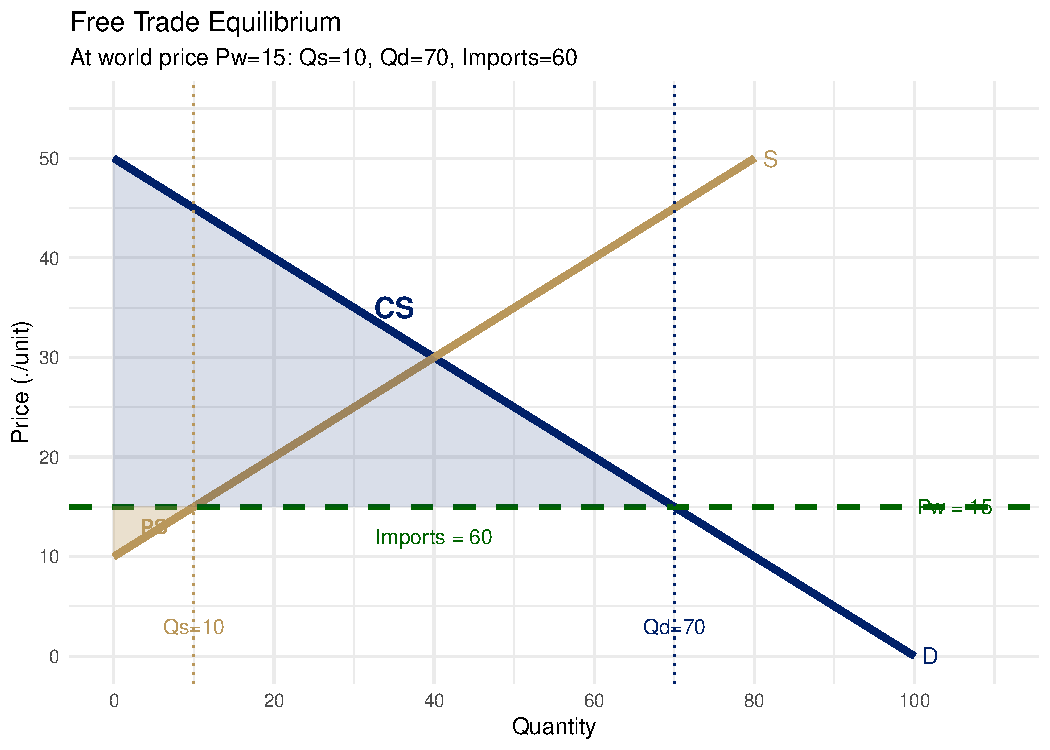
\includegraphics[keepaspectratio]{Lecture07_Protectionism_I_files/figure-beamer/fig-free-trade-1.pdf}}

}

\caption{\label{fig-free-trade}Free Trade: Domestic Supply, Demand, and
World Price Source: Author's illustration.}

\end{figure}%

\textbf{Free trade baseline:} \(D: P = 50 - Q/2\) · \(S: P = 10 + Q/2\)
· \(P_w = 15\)

At \(P_w=15\): domestic supply \(Q_s=10\), domestic demand \(Q_d=70\),
\textbf{imports = 60 units}.
\end{block}
\end{frame}

\begin{frame}
\begin{block}{Partial Equilibrium Analysis of a Tariff}
\phantomsection\label{partial-equilibrium-analysis-of-a-tariff}
\textbf{Free trade equilibrium at \(P_w\):} Domestic supply \(Q_s^0\);
domestic demand \(Q_d^0\); imports \(M_0 = Q_d^0 - Q_s^0\)

\textbf{After tariff \(t\): domestic price → \(P_w + t\):} Domestic
supply rises: \(Q_s^1 > Q_s^0\); demand falls: \(Q_d^1 < Q_d^0\);
imports fall: \(M_1 = Q_d^1 - Q_s^1 < M_0\)

\textbf{Welfare triangles:}

\begin{longtable}[]{@{}ll@{}}
\toprule\noalign{}
Effect & Direction \\
\midrule\noalign{}
\endhead
Consumer surplus & ↓ (trapezoid \emph{A+B+C+D}) \\
Producer surplus & ↑ (rectangle \emph{A}) \\
Govt revenue & ↑ (rectangle \emph{C}) \\
{Deadweight loss} & ↑ (triangles \emph{B + D}) \\
\bottomrule\noalign{}
\end{longtable}

\textbf{Triangle \emph{B}} = production distortion loss (resources
diverted to inefficient domestic production)

\textbf{Triangle \emph{D}} = consumption distortion loss (consumers
priced out of market)

Both are pure efficiency loss.
\end{block}
\end{frame}

\begin{frame}
\begin{block}{Effect of a Tariff --- Welfare Analysis}
\phantomsection\label{effect-of-a-tariff-welfare-analysis}
\begin{figure}

\centering{

\pandocbounded{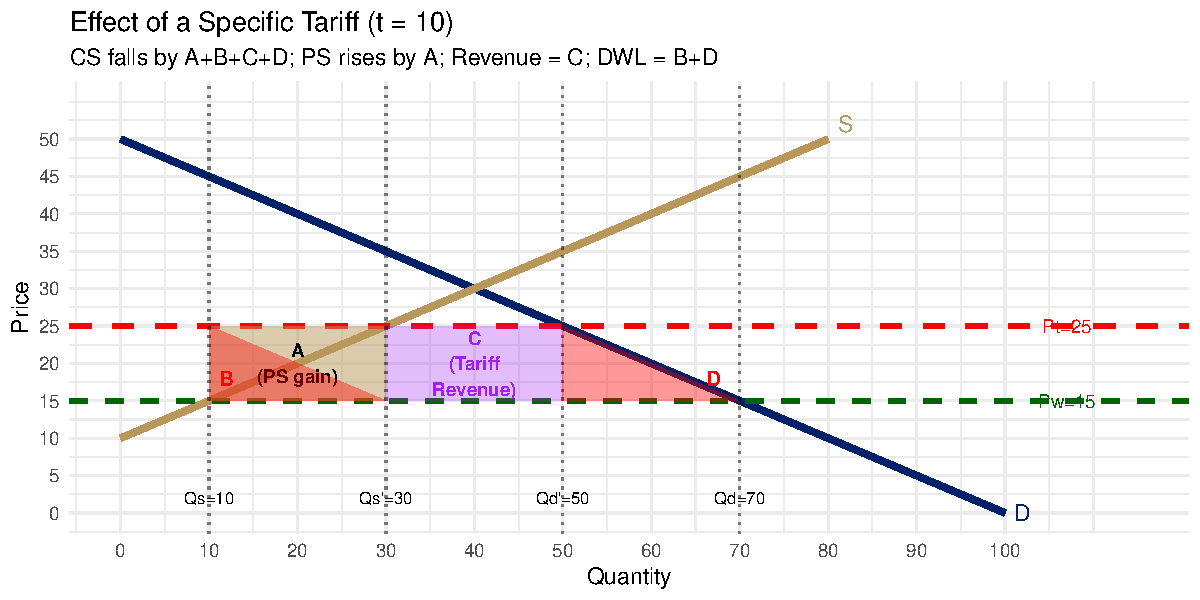
\includegraphics[keepaspectratio]{Lecture07_Protectionism_I_files/figure-beamer/fig-tariff-welfare-1.pdf}}

}

\caption{\label{fig-tariff-welfare}Specific Tariff t=10: CS Lost, PS
Gained, DWL Triangles Source: Author's illustration.}

\end{figure}%
\end{block}
\end{frame}

\begin{frame}
\begin{block}{Welfare Accounting: The Tariff Identity}
\phantomsection\label{welfare-accounting-the-tariff-identity}
\[\Delta CS = -(A + B + C + D)\]

\[\Delta PS = +A\]

\[\text{Tariff Revenue} = +C\]

\[\boxed{\Delta \text{National Welfare} = -(B + D)}\]

Where:

\begin{itemize}
\tightlist
\item
  \textbf{B} = \emph{production distortion loss} --- resources
  wastefully drawn into domestic production
\item
  \textbf{D} = \emph{consumption distortion loss} --- consumers
  wastefully priced out of the market
\end{itemize}

\textbf{For a small country:} the tariff always reduces national welfare
by the deadweight loss triangles \(B + D\).

\textbf{Numerical example:} With \(t=10\), \(P_w=15\): -
\(\Delta CS = -(A+B+C+D)\);
\(B = \tfrac{1}{2}(30{-}10)(25{-}15) = 100\);
\(D = \tfrac{1}{2}(70{-}50)(25{-}15) = 100\) -
\(B = \frac{1}{2}(30-10)(25-15) = 100\);
\(D = \frac{1}{2}(70-50)(25-15) = 100\); \textbf{DWL = 200}
\end{block}
\end{frame}

\begin{frame}
\begin{block}{Winners and Losers from a Tariff}
\phantomsection\label{winners-and-losers-from-a-tariff}
\begin{longtable}[]{@{}
  >{\raggedright\arraybackslash}p{(\linewidth - 4\tabcolsep) * \real{0.3333}}
  >{\raggedright\arraybackslash}p{(\linewidth - 4\tabcolsep) * \real{0.3333}}
  >{\raggedright\arraybackslash}p{(\linewidth - 4\tabcolsep) * \real{0.3333}}@{}}
\toprule\noalign{}
\begin{minipage}[b]{\linewidth}\raggedright
Group
\end{minipage} & \begin{minipage}[b]{\linewidth}\raggedright
Effect
\end{minipage} & \begin{minipage}[b]{\linewidth}\raggedright
Reason
\end{minipage} \\
\midrule\noalign{}
\endhead
{Domestic producers} & \textbf{Gain} & Higher domestic price, expand
output \\
{Consumers} & \textbf{Lose} & Pay higher price, consume less \\
{Government} & \textbf{Gain revenue} & Tariff × import volume \\
\textbf{Net welfare (small country)} & \textbf{Loss} & DWL = \emph{B +
D} \\
\bottomrule\noalign{}
\end{longtable}

\textbf{Small country assumption:} Country is a price taker --- the
tariff does not affect the world price.

\textbf{Large country exception:} If India's import demand is large
enough to move world prices, a tariff can improve India's \emph{terms of
trade} → \textbf{optimal tariff} (see later).
\end{block}
\end{frame}

\begin{frame}
\begin{block}{India's Agricultural Tariff Structure}
\phantomsection\label{indias-agricultural-tariff-structure}
\textbf{WTO commitments (FY2024):}

\begin{longtable}[]{@{}lll@{}}
\toprule\noalign{}
& Bound & Applied \\
\midrule\noalign{}
\endhead
All goods & 48.5\% & 13.8\% \\
Agriculture & \textbf{113.5\%} & \textbf{36.4\%} \\
\bottomrule\noalign{}
\end{longtable}

``\textbf{Water in the tariff}'' = gap between bound and applied rates.
India retains large room to raise tariffs without breaching WTO
commitments.

\textbf{Selected high-tariff items:}

\begin{longtable}[]{@{}ll@{}}
\toprule\noalign{}
Commodity & Applied duty \\
\midrule\noalign{}
\endhead
Palm oil & 100\% (basic + AIDC) \\
Sugar & 100\% \\
Wheat & 50\% \\
Maize & 60\% \\
Milk (SMP) & 60\% \\
\bottomrule\noalign{}
\end{longtable}

India's bound rate of \textasciitilde114\% is one of the \textbf{highest
among G20 nations} for agriculture.
\end{block}
\end{frame}

\begin{frame}
\begin{block}{India's Agricultural Tariff Profile}
\phantomsection\label{indias-agricultural-tariff-profile}
\begin{figure}

\centering{

\pandocbounded{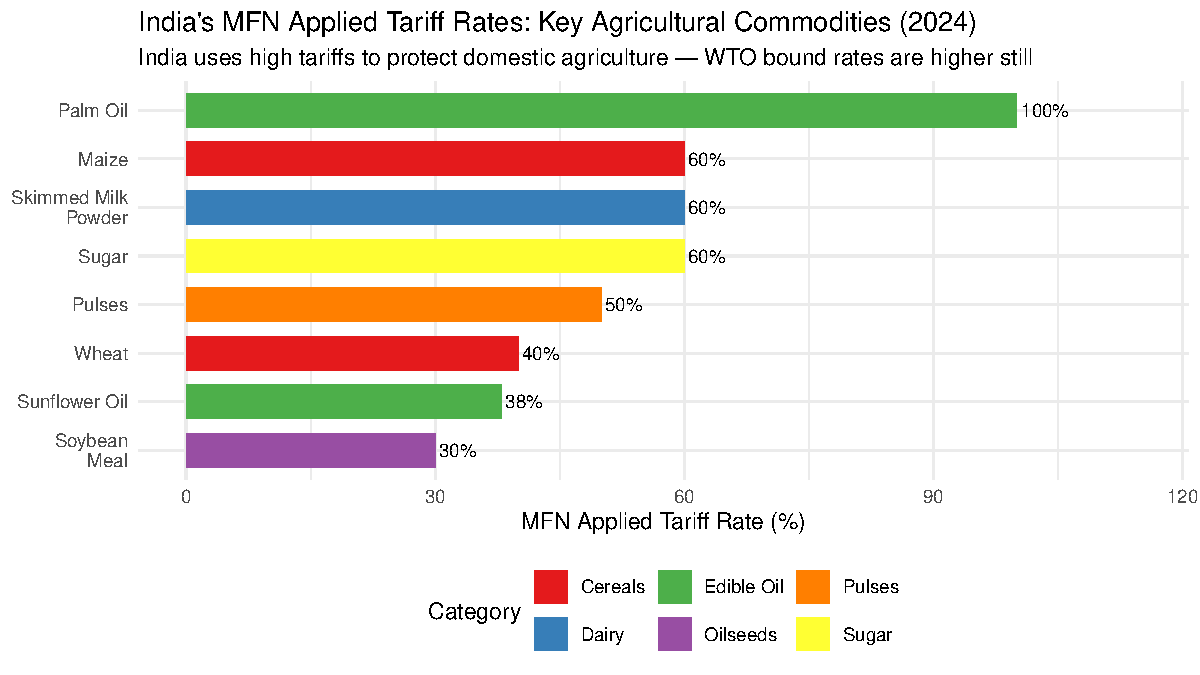
\includegraphics[keepaspectratio]{Lecture07_Protectionism_I_files/figure-beamer/fig-india-tariffs-1.pdf}}

}

\caption{\label{fig-india-tariffs}India: Applied MFN Tariff Rates on Key
Agricultural Imports (2024) Source: WTO, Tariff Profiles (2024); DGFT.}

\end{figure}%
\end{block}
\end{frame}

\begin{frame}
\begin{block}{The Tariff Rate Quota (TRQ)}
\phantomsection\label{the-tariff-rate-quota-trq}
A \textbf{TRQ} combines two tariff levels:

\begin{enumerate}
\tightlist
\item
  \textbf{Within-quota tariff (low):} applies to a fixed import volume
\item
  \textbf{Over-quota tariff (high):} applies to imports beyond the quota
\end{enumerate}

\textbf{Effect:} Allows \emph{some} imports cheaply (food security)
while discouraging \emph{large} imports (protects producers).

\textbf{India's TRQs under WTO AoA:}

\begin{longtable}[]{@{}lll@{}}
\toprule\noalign{}
Commodity & In-quota duty & Over-quota \\
\midrule\noalign{}
\endhead
Maize & 15\% & 60\% \\
Skimmed milk & 15\% & 60\% \\
Crude soybean oil & 45\% & 100\% \\
\bottomrule\noalign{}
\end{longtable}

TRQs were bound at Uruguay Round (1994). India rarely fills its TRQ
allocations.
\end{block}
\end{frame}

\begin{frame}
\begin{block}{Case Study: India's Palm Oil Import Duty}
\phantomsection\label{case-study-indias-palm-oil-import-duty}
\textbf{Timeline:}

\begin{itemize}
\tightlist
\item
  \textbf{2017:} Basic duty 0\% (edible oil prices rising)
\item
  \textbf{2020:} Raised to 37.5\% (protecting oilseed farmers)
\item
  \textbf{2021:} Basic + AIDC + SWS ≈ \textbf{100\%} effective duty
\end{itemize}

\textbf{Rationale:} Protect domestic oilseed farmers (soybean,
groundnut, mustard).

\textbf{The dilemma:} India imports \textbf{\textasciitilde14 million
tonnes/year} of edible oils --- 60\% of consumption. Cannot substitute
quickly. Farmers in MP, Rajasthan gain; urban consumers lose; food
inflation rises.

\textbf{Terms of trade argument partially valid:} India is the world's
largest palm oil importer --- its import demand moves global prices. A
tariff improves India's ToT at the cost of Malaysian/Indonesian
exporters.
\end{block}
\end{frame}

\begin{frame}
\begin{block}{Effective Rate of Protection (ERP)}
\phantomsection\label{effective-rate-of-protection-erp}
\textbf{Nominal tariff} = tariff on the final good. \textbf{ERP} =
protection on \emph{value added} in production, accounting for tariffs
on \emph{inputs}.

\[\text{ERP} = \frac{t_f - \sum a_i t_i}{1 - \sum a_i}\]

where \(t_f\) = nominal tariff on final good, \(t_i\) = tariff on input
\(i\), \(a_i\) = input share in value.

\textbf{Example: Sugar processing}

\begin{itemize}
\tightlist
\item
  Tariff on sugar (final): 100\%; tariff on sugarcane (input): 0\%;
  input share: \textasciitilde70\%
\end{itemize}

\[\text{ERP} = \frac{0.10 - 0}{1 - 0.70} \approx 333\%\]

\textbf{ERP \textgreater\textgreater{} nominal tariff} = ``tariff
escalation'' --- processing stages protected far more than raw material.

India's tariff structure commonly exhibits cascading --- protecting
processing industries at the expense of downstream consumers and raw
material exporters.
\end{block}
\end{frame}

\begin{frame}{Part II: Quotas}
\phantomsection\label{part-ii-quotas}
\end{frame}

\begin{frame}
\begin{block}{What is an Import Quota?}
\phantomsection\label{what-is-an-import-quota}
A \textbf{quota} is a quantitative restriction --- it sets the
\emph{maximum volume} of a good that may be imported in a given period.

\textbf{How it works:}

\begin{enumerate}
\tightlist
\item
  Government announces quota (e.g., 1 million tonnes of wheat)
\item
  Import licences issued (to traders, state agencies, or by auction)
\item
  Once quota filled, further imports blocked
\item
  Domestic price rises until supply + quota = demand
\end{enumerate}

\textbf{Quota rent:} The gap between domestic and world price × quota
volume = \textbf{quota rent}. Who captures the rent? If licences
\textbf{auctioned} → government; if licences \textbf{given away} →
importers (or exporters under VER).
\end{block}
\end{frame}

\begin{frame}
\begin{block}{Import Quota --- Same Effect, Different Mechanism}
\phantomsection\label{import-quota-same-effect-different-mechanism}
\begin{figure}

\centering{

\pandocbounded{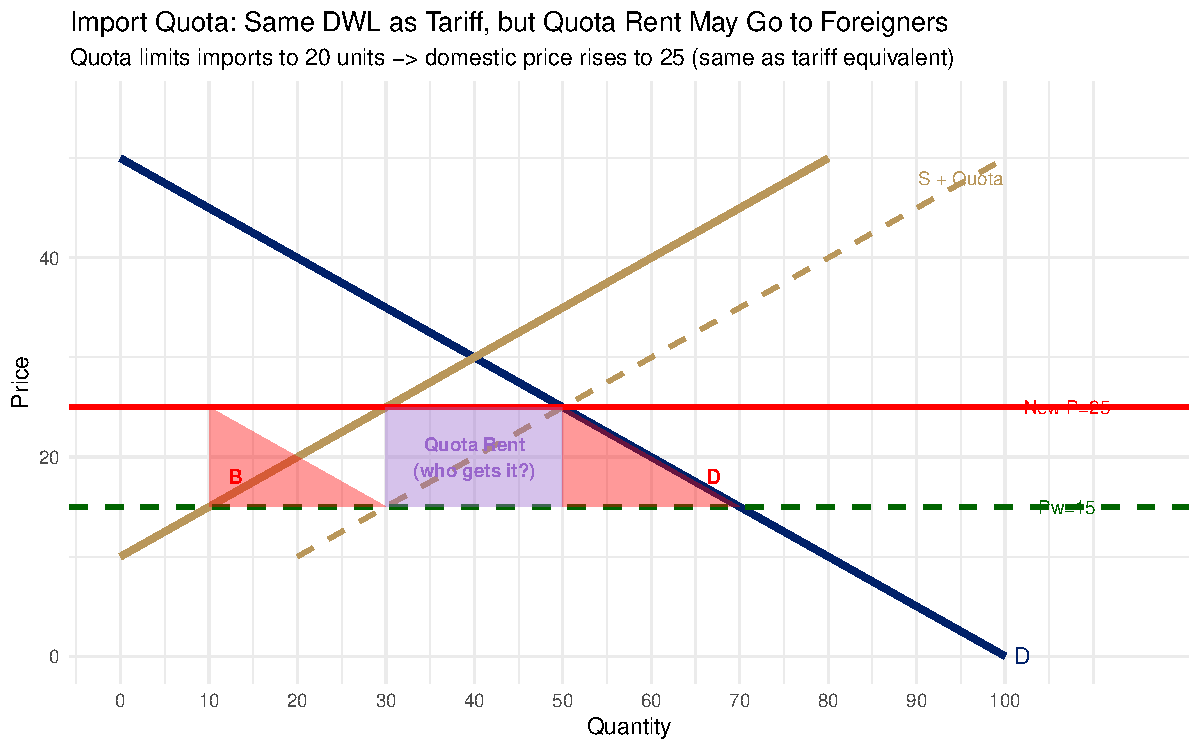
\includegraphics[keepaspectratio]{Lecture07_Protectionism_I_files/figure-beamer/fig-quota-1.pdf}}

}

\caption{\label{fig-quota}Import Quota: Quantity Restriction Creates
Quota Rent Instead of Revenue Source: Author's illustration.}

\end{figure}%
\end{block}
\end{frame}

\begin{frame}
\begin{block}{Tariff vs Quota: Revenue vs Rent}
\phantomsection\label{tariff-vs-quota-revenue-vs-rent}
\textbf{Key difference in revenue allocation:}

\[\text{Tariff: Revenue} = t \times M \quad \text{(goes to government)}\]

\[\text{Quota: Rent} = (P_t - P_w) \times \bar{M} \quad \text{(may go to foreign exporters)}\]

\textbf{When quota rent goes to foreigners:} If import licences are
given free to foreign exporters (as in a VER), the domestic economy
loses the tariff-equivalent rectangle \emph{C}. Net welfare loss =
\(B + C + D\) \textgreater{} tariff welfare loss of \(B + D\).

\textbf{When quota rent stays domestic:} If licences are
\emph{auctioned} to domestic importers, the domestic economy captures
rent = equivalent to tariff.

\textbf{Implication for policy:} If quota rents accrue to foreign
exporters, quotas are \textbf{worse than equivalent tariffs} --- the
domestic economy loses both the DWL and the revenue. This is why
economists generally prefer tariffs over quotas, and why WTO's GATT
Article XI prohibits quotas.
\end{block}
\end{frame}

\begin{frame}
\begin{block}{Tariff vs Quota: Similarities and Differences}
\phantomsection\label{tariff-vs-quota-similarities-and-differences}
\begin{longtable}[]{@{}
  >{\raggedright\arraybackslash}p{(\linewidth - 4\tabcolsep) * \real{0.3333}}
  >{\raggedright\arraybackslash}p{(\linewidth - 4\tabcolsep) * \real{0.3333}}
  >{\raggedright\arraybackslash}p{(\linewidth - 4\tabcolsep) * \real{0.3333}}@{}}
\toprule\noalign{}
\begin{minipage}[b]{\linewidth}\raggedright
Feature
\end{minipage} & \begin{minipage}[b]{\linewidth}\raggedright
Tariff
\end{minipage} & \begin{minipage}[b]{\linewidth}\raggedright
Quota
\end{minipage} \\
\midrule\noalign{}
\endhead
Domestic price & Rises & Rises \\
Domestic production & Rises & Rises \\
Imports & Fall & Fall (fixed) \\
Government revenue & \textbf{Yes --- tariff revenue} & Only if licences
auctioned \\
Flexibility under demand shock & Adjusts automatically & Quantity fixed
--- price volatile \\
Transparency & More transparent & Less --- hidden in licensing \\
WTO legality & Bound and transparent & Mostly prohibited (GATT Art
XI) \\
\bottomrule\noalign{}
\end{longtable}

\textbf{Key asymmetry:} Under a tariff, if demand rises, imports rise
(at fixed tariff price). Under a quota, imports are fixed --- domestic
price must rise to clear the market. Quotas are more price-volatile and
less transparent.
\end{block}
\end{frame}

\begin{frame}
\begin{block}{India's Quantitative Restrictions: History}
\phantomsection\label{indias-quantitative-restrictions-history}
\textbf{Pre-2001:} India maintained extensive QRs on agricultural
imports citing \textbf{balance of payments} reasons (GATT Article
XVIII:B) --- QRs on hundreds of agricultural product lines; effective
near-ban on many imports.

\textbf{2001:} USA challenged India's QRs at WTO. \textbf{Panel ruling:}
India's BoP situation no longer justified QRs. India removed most
agricultural QRs.

\textbf{Post-2001 shift:} India replaced QRs with \textbf{high tariffs}
--- achieving similar protection through a WTO-consistent instrument.
``Tariffication'' converted quantity restrictions to price restrictions.
Tariff flexibility (``water'') provides buffer for future protection.
\end{block}
\end{frame}

\begin{frame}
\begin{block}{The Optimal Tariff Argument}
\phantomsection\label{the-optimal-tariff-argument}
For a \textbf{large country}, an import tariff reduces demand for
imports → world price falls → terms of trade improve.

\textbf{Optimal tariff} = tariff that maximises net welfare gain:

\[t^* = \frac{1}{\varepsilon_x^*}\]

where \(\varepsilon_x^*\) = foreign export supply elasticity. More
inelastic foreign supply → higher optimal tariff.

\textbf{India's case (palm oil):} India = 15\% of world palm oil demand.
Malaysian/Indonesian export supply somewhat inelastic → India can
depress world palm oil prices with a tariff → Terms of trade gain
partially offsets DWL.

\textbf{Caveat:} Retaliation risk. If Malaysia retaliates on Indian
exports (spices, pharmaceuticals), net welfare impact uncertain.

\textbf{Optimal tariff is the only trade-restriction argument that
raises national welfare in economic theory} --- and only for large
countries.
\end{block}
\end{frame}

\begin{frame}
\begin{block}{Infant Industry Protection: India's Experience}
\phantomsection\label{infant-industry-protection-indias-experience}
\textbf{Argument:} A nascent domestic industry cannot compete initially
due to high startup costs, lack of accumulated learning-by-doing, and
missing domestic supply chains. \textbf{Temporary} protection allows the
industry to mature → eventually competitive.

\textbf{Post-Independence India:} Bombay Plan (1944) --- protect
everything. Led to License Raj.

\textbf{Agriculture examples:}

\begin{itemize}
\tightlist
\item
  \textbf{Green Revolution:} seed, fertiliser, irrigation subsidised →
  Indian wheat/rice went from deficit to surplus
\item
  \textbf{Oilseeds:} Technology Mission on Oilseeds (1986) used tariff +
  R\&D → raised productivity
\item
  \textbf{Sugar:} Protected since 1932 --- never ``grown up.'' Chronic
  intervention = perennial inefficiency.
\end{itemize}

\textbf{Key insight:} Protection that never ends becomes a permanent
rent transfer from consumers to producers, not an investment in future
competitiveness.
\end{block}
\end{frame}

\begin{frame}
\begin{block}{Voluntary Export Restraints (VERs)}
\phantomsection\label{voluntary-export-restraints-vers}
A \textbf{VER} occurs when an exporting country ``voluntarily''
restricts its exports to a trading partner --- usually under diplomatic
pressure.

\textbf{Classic example:} Japan limited auto exports to USA in the
1980s. \textbf{Effect:} Like a quota but the \emph{quota rent accrues to
the exporter} (not the importer government). \textbf{WTO:} VERs are now
illegal under Article 11 of WTO Safeguards Agreement (post-Uruguay
Round).

\textbf{India-adjacent example:} India's 2023 rice export restrictions
raised world prices --- effectively a VER from the perspective of
importing nations like Bangladesh, Benin, and Senegal. India's rice
export controls demonstrated India's market power as the world's
dominant rice exporter.
\end{block}
\end{frame}

\begin{frame}
\begin{block}{Non-Tariff Barriers (NTBs): Preview}
\phantomsection\label{non-tariff-barriers-ntbs-preview}
\textbf{NTBs} are behind-the-border measures that restrict trade without
an explicit tariff or quota:

\begin{itemize}
\tightlist
\item
  \textbf{SPS (Sanitary \& Phytosanitary):} food safety, animal/plant
  health standards
\item
  \textbf{TBT (Technical Barriers to Trade):} labelling, packaging,
  quality standards
\item
  \textbf{Licensing requirements; customs procedures and delays; state
  trading monopolies}
\end{itemize}

\textbf{The ``new protectionism'':} As tariffs have fallen under WTO,
NTBs have risen to replace them. India's rejection of GM soybean imports
(SPS), EU's pesticide MRLs on Indian spices, and USA's countervailing
duties on Indian shrimp are all NTB-related disputes.

\textbf{Detailed treatment: Lecture 15.}
\end{block}
\end{frame}

\begin{frame}
\begin{block}{Summary: Tariffs and Quotas}
\phantomsection\label{summary-tariffs-and-quotas}
\textbf{Core findings:}

\begin{enumerate}
\item
  \textbf{Tariffs} raise domestic prices, protect producers, generate
  government revenue, but impose deadweight losses \(B + D\) on the
  economy.
\item
  \textbf{Quotas} have similar price effects but create quota rents
  (often captured by private importers or foreign exporters) and are
  more price-volatile.
\item
  India uses \textbf{high bound tariffs as a buffer} --- ``water in the
  tariff'' provides policy space without WTO violation.
\item
  The \textbf{ERP} often exceeds the nominal tariff due to tariff
  escalation in India's structure.
\item
  \textbf{Optimal tariff} is the only theoretically valid
  welfare-raising argument --- and only for large countries like India
  in palm oil.
\end{enumerate}

\note{\begin{enumerate}
\setcounter{enumi}{5}
\tightlist
\item
  Welfare identity: \(\Delta W = -(B+D)\) for small country; may be
  positive for large country at optimal tariff.
\end{enumerate}}

\textbf{India's agricultural protection architecture:} High applied
tariffs + TRQs + licensing + SPS/NTBs = multi-layered protection. WTO
constraints bind only at the margins.
\end{block}
\end{frame}

\begin{frame}
\begin{block}{Next Lecture}
\phantomsection\label{next-lecture}
\textbf{Lecture 8 --- Protectionism II: Subsidies, Dumping \& Cartels}
\emph{June 16, 2026}

\begin{itemize}
\tightlist
\item
  Export subsidies and their effects on world markets
\item
  India's MSP and WTO's Amber Box rules
\item
  Fertiliser subsidies and trade distortion
\item
  Dumping: definition, types, anti-dumping duties
\item
  India as the world's top anti-dumping user
\item
  Agricultural cartels and commodity agreements
\item
  India's rice export ban (2023) as market power exercise
\end{itemize}

\textbf{Preparation:} Read Krugman, Obstfeld \& Melitz, Ch. 9 (Export
Subsidies and Import Quotas). Review India's WTO notification on
domestic support (2022).
\end{block}
\end{frame}

\begin{frame}{Appendix}
\phantomsection\label{appendix}
\begin{block}{Additional Resources}
\phantomsection\label{additional-resources}
\textbf{Further Reading}

\begin{itemize}
\tightlist
\item
  \emph{International Economics} --- Salvatore (Ch. 9-11)
\item
  \emph{International Economics} --- Appleyard \& Field (Ch. 9-11)
\item
  RBI/DGCI\&S/APEDA databases for latest data
\end{itemize}

\textbf{Key Data Sources}

\begin{itemize}
\tightlist
\item
  DGCI\&S: India's merchandise trade
\item
  RBI: Balance of payments data\\
\item
  APEDA: Agricultural export statistics
\item
  WTO: Tariff and trade databases
\end{itemize}
\end{block}
\end{frame}




\end{document}
